\documentclass[12pt]{article}
\usepackage{graphicx}
\usepackage{amsmath}
\usepackage{amssymb}
\usepackage[authoryear]{natbib}
\usepackage{enumerate}
\usepackage{booktabs}
\usepackage{siunitx}
\newcolumntype{d}{S[
      input-open-uncertainty=,
      input-close-uncertainty=,
      parse-numbers = false,
      table-align-text-pre=false,
      table-align-text-post=false
    ]}
\usepackage{pdflscape}
\usepackage{hyperref}

\hypersetup{
    colorlinks,
    citecolor=black,
    filecolor=black,
    linkcolor=black,
    urlcolor=black
}
\setlength{\parindent}{0pt}
\usepackage[parfill]{parskip}
\date{Lent 2023}
\title{Dissertation draft}
\author{Tobias Leigh-Wood}
\usepackage[letterpaper, margin=1.1in]{geometry}
\linespread{1.1}

\begin{document}

\maketitle
\tableofcontents
\newpage

Standard economic theory suggests that retirement annuities, which provide a guaranteed income stream until the end of life,
should be highly valued by individuals as a way to insure against late death \cite{yaari_65}. However, in developed countries,
rates of annuitisation are far below the levels that theory predicts. The literature has suggested several reasons for
this, but there is no consensus about which mechanism is dominant. I exploit early retirees' consumption responses to a
reform to annuity policy in the UK to add to this literature.
    [\textbf{Add something once I have a conclusion}].

In the UK, adults have three methods of funding retirement: the state pension; defined benefit (DB) employee pension schemes,
which provide an income in retirement based on years of service and a function of wages; and defined contribution (DC) pensions,
in which individuals save and invest in a tax-advantaged account that is usually supplemented with employer contributions.
Under the 2010-2015 coalition government in the UK, the law regarding the use of private DC pensions at
retirement changed. Individuals were no longer forced to annuitise, which provides a constant income until death,
their pension pots and could access them in a variety of ways such as a lump sum withdrawal or income drawdown,
which is a steady withdrawal of assets
with the remainder left in the pot - common advice is to take 4\% a year.
Subsequently the number of annuities sold in the UK dropped precipitously.

In this paper, I first use the policy reform as a discontinuity to measure the impact of forced annuitisation on the consumption
levels of individuals in the first few years of retirement. Given that the reform was implemented suddenly and without
advanced notice before the Spring 2014 budget, I claim that individuals who retired in 2015, 2016 or 2017
are otherwise similar to those who retired year in 2011, 2012 and 2013 except for the fact the later retirees
do not need to annuitise their DC pension pots. Therefore, I can use a regression discontinuity to identify
the effect that forced annuitisation has on the consumption of retirees.

I then test two competing hypotheses for the annuity puzzle: bequests and
pessimistic life expectancy. The annuity puzzle was first identified by \cite{yaari_65} and is a classed as a problem
since standard economic theory cannot explain the lack of annuitisation that is observed in the real world.
Two possible explanations are bequests and life expectancy: individuals want to leave an estate for their heirs to
inherit and they cannot do this if they annuitise their wealth; or individuals may believe they will not live
as long as annuity providers think they will and therefore annuities that are on the market do not appear to be
good value. Depending on which reason explains the lack of annuitisation in the UK, the consumption response of
retirees to the pension
reform will differ. If individuals do not annuitise because of pessimistic life expectancy their
consumption should increase after the reform. If, on the other hand, individuals do not annuitise because of a bequest motive, consumption
should not change much as a result of the reform.

I will solve lifecycle models
(\textbf{maybe add something about lifecycle models here})
for both of these cases and simulate
consumption decisions with and without forced annuitisation. I will then use a variety of empirical models to measure
the consumption change in early retirement that resulted from the policy reform. The sign and magnitude of this change
will be indicative of the mechanism causing the annuitisation problem.


The importance of retirement policy to individuals in the UK is growing. The number of individuals of
pensionable age is expected to increase from 11.9 million in 2020 to 15.2 million in
2045 according to the latest Office for National Statistics (ONS) and for every 1000 people of working age there will be 341 of pensionable
age in 2045 compared to 280 in 2020 \cite{ons_population_predictions_2020}. The increase in absolute and relative
numbers of elderly people makes retirement policy more consequential. Moreover, private DC pensions are
becoming increasingly common and are predicted to grow as current cohorts age \cite{cribb_karjalainen_ifs_2023}.
Therefore, policies regarding how private pensions can be accessed will have a larger impact on overall welfare for
retirees.

Moreover, understanding how retirees spend their money over retirement is an important policy question of its own.
If retirees spend too much in early retirement, the state may need to provide for them towards the end of their
lives. This has implications for government budgets, especially since population aging means more individuals will
require expensive end of life care. On the other hand, if retirees over-save and do not spend, the economy may face
a dynamic inefficiency whereby consumption per capita could be increased if savings were decreased. (Get dynamic inefficiency
reference.)


\subsection{Literature review}
My paper builds on three main strands of literature: that of the annuity puzzle, exploring reasons that some retirees choose not to annuitise;
the retirement saving puzzle, looking at consumption and saving behaviour over retirement; and lifecycle models, whereby the above
problems are explained using a tractable model of human decision making.

\cite{yaari_65} was the first to show that under standard assumptions we would expect individuals to
annuitise all of their wealth at retirement to insure against the risk of long life. Since then there
has been much literature discussing possible reasons that people do not annuitise. \cite{finkelstein_porteba_2002}
and \cite{finkelstein_porteba_2004} find evidence of adverse selection, thereby making the 'money's worth'
of annuities lower for the general population as opposed to the population of annuitants. However, they
also find that theory would still predict annuitisation.

\cite{friedman_warshawsky_qje_1990} show that annuitisation decisions can be fully explained by a mixture of
bequest motives and actuarily unfair annuities. They solve an augmented life-cycle model with a range of
parameters on how severe the rate of return is on the annuity versus market rates. For plausible values
they find that individuals would optimally not annuitise much wealth. Similarly to \cite{finkelstein_porteba_2004},
\cite{friedman_warshawsky_chicago_1988} show that there is a significant difference between the life expectancy of
annuitants and the general population in the American annuity market but this cannot fully explain the annuitisation
puzzle. Only when bequest motives are added to the model can annuitisation rates be rationalized.

\cite{lockwood_red_2012} builds on this and shows that a realistic bequest motive in lifecycle simulations achieves
realistic annuitisation rates. He solves a simple lifecycle model with bequest motives taken from several recent papers
in the literature. The bequest motives he picks therefore match other important aspects of the lifecycle model such
as how much individuals actually bequest and how rich individuals are when they bequest.

\cite{lockwood_aer_2018}

\cite{vidalmelia_lejarragagarcia_munich_2004} have some interesting results. Need to talk about that.

\textbf{If I add 300 more words here then I will be at 5000!}

\textbf{There are some more papers I will include here.}

\section{Data and Policy reform}

\subsection{Data}

The main data set I use is the English Longitudinal Study of Ageing (ELSA) \cite{main_elsa_citation}. ELSA picks individuals
over the age of 50 to survey every two years until death. If individuals leave the survey ELSA replaces them so that it is
representative of the over 50 population in the UK. Individuals are asked a range of questions relating to their income
and wealth as well as expectations about the future. One benefit of using ELSA is that it includes data on pension types
for individuals who are working. Therefore, I can differentiate between individuals who have a DC pension and those who have a DB pension.
There have been 9 waves of ELSA data collection, the first was in 2001 and collections happened every two years thereafter.

Importantly ELSA also includes information on pension size that the Institute for Fiscal Studies (IFS) calculated, this is only available
up until wave 5 (which was collected in 2010 and 2011) at which point I use a real return
of 3\% to predict forward the pension wealth variable until retirement. ELSA also includes a measure of all
non-housing financial wealth which I use in some specifications because of these issues with
pension wealth. Due to slight differences in the ELSA questions between years, I use `Harmonized ELSA'
\footnote{This analysis uses data or information from the Harmonized ELSA dataset and Codebook, Version G.2 as of
    July 2021 developed by the Gateway to Global Aging Data. The development of the Harmonized ELSA was funded by the National
    Institute on Aging (R01 AG030153, RC2 AG036619, R03 AG043052). For more information,
    please refer to https://g2aging.org/.} which ensures that variables are comparable across waves. Since this only includes a
subset of the questions in ELSA, I also supplement it with variables taken directly from the data such as questions that deal
with life expectancy.

ELSA also includes questions on expenditures. In particular, individuals are asked how much they consume across a range of broad
categories including in-house food consumption, out-of-house food consumption, leisure consumption, clothes consumption and
consumption on utility bills and rent. I use also use two variables related to life expectancy that I discuss in more detail below.

I also use `life tables' from the UK's ONS. These provide me with risk of death for each age group. I adjust them
to make death certain at age 110 as is common in the literature. I transform these so that I have risk of death conditional on being
a given age since this is what I use in the life cycle simulations. I also use these objective probabilities to
calculate annuity prices for individuals.

To illustrate the effect the reform had on sales of annuities in the UK I obtained product data from the Financial Conduct Authority.
These track the sales of different financial products overtime including data annuities.

Life expectancy impacts decision to retire for two reasons. Firstly, it directly impacts the price that an annuity will cost for
individuals. Older individuals and those with pre-existing health conditions generally can buy an annuity that provides a greater
income stream than individuals who are younger. Secondly, private information about life expectancy impacts the perceived
value of an annuity. If an individual expects to outlive the general population an annuity, at a given price, will appear
a much better deal to them. Likewise, an individuals life expectancy will change their decision on how to consume and save
through retirement.

To calculate subjective life expectancies I follow \cite{odea_sturrock_rest_2023}. Individuals are asked “What are the chances that you will
live to be age X or more?” where X changes depending on the age of the interviewee. If individuals were under 65 then X was 75, if individuals
were 66 and older they were asked the age that was 11 to 15 years older than them and is a multiple of 5. From wave three respondents were
also asked “What are the chances that you will live to be age 85 or more?” if they were under 70. As most recent retirees are under 70 we
therefore have two data points. I first drop from the data individuals who think it is more likely that they reach a higher age than a younger
age since this shows a misunderstanding of the question. I then add as a third data point their objective chance of reaching 110 according to the ONS life tables.
I fit these three points to a Weibull distribution, which is commonly used by demographers to estimate how populations
will age, using non-linear least squares. Then I create subjective survival tables using parameters from the Weibull distribution.

\textbf{I could go into more detail here? Maybe I should. Add equation etc}


\subsection{Policy reform}

Successive governments in the UK have attempted to reform both the public and private pension system. Prior
to 1987, participation in private schemes was limited to employees of firms that had offered them, and there
were few alternatives to the public state pension or defined benefit scheme that a public sector employer
would offer. From 1989, individuals in the UK were allowed to open tax advantaged self-invested personal pensions
alongside any pension their employer offered. The 2004 Finance Act rationalised taxation rates on different types of pensions.
But DC pension pots could still only be used to buy an annuity after taking out a maximum of 25\% as a tax free lump sum withdrawal
from age 55 onwards. Most pension pots also required that individuals access them before age 75.

Announced in the spring budget of 2014, the so called `pensions freedom act' received Royal Asset in December 2014 marked the end of a series
of pension reforms carried out by the coalition government between 2010 and 2015. The reform made it possible
to withdraw the first 25\% from a pension pot tax free and the rest subject to the marginal rate of income tax that an individual faced.
In the June 2010 budget, the government made a first reform to the annuitisation rules, creating
a minimum income requirement above which individuals would not need to
annuitise more \cite{finance_act_hmt_2011} (this meant high income retirees would not need to annuitise their wealth).
However, this was set at £20,000 and therefore few individuals
were eligible. The minimum income requirement was scrapped in the 2014 bill, finally eliminating the
compulsory annuities market, with one government minister saying pension pots `can be used to buy Lamborghinis'
\cite{guardian_lambos}.

The impact of the reforms on annuity demand has been documented by \cite{cannon_et_al_nier_2016}.
Using data from the Association of British Insurers, they show that annuity demand dropped by 75\% from
its maximum in 2011
\textbf{Check}
. Figure \ref{fig:annovertime} shows purchases of annuities overtime and demonstrates the sharp decrease
in purchases that happened from 2014 to 2015. There was an increase in the number of pensions that were
being accessed using an income drawdown product, but these do not fully account for the drop in annuitisation.
\begin{figure}[h]
    \caption{Pension pots accessed }
    \centering
    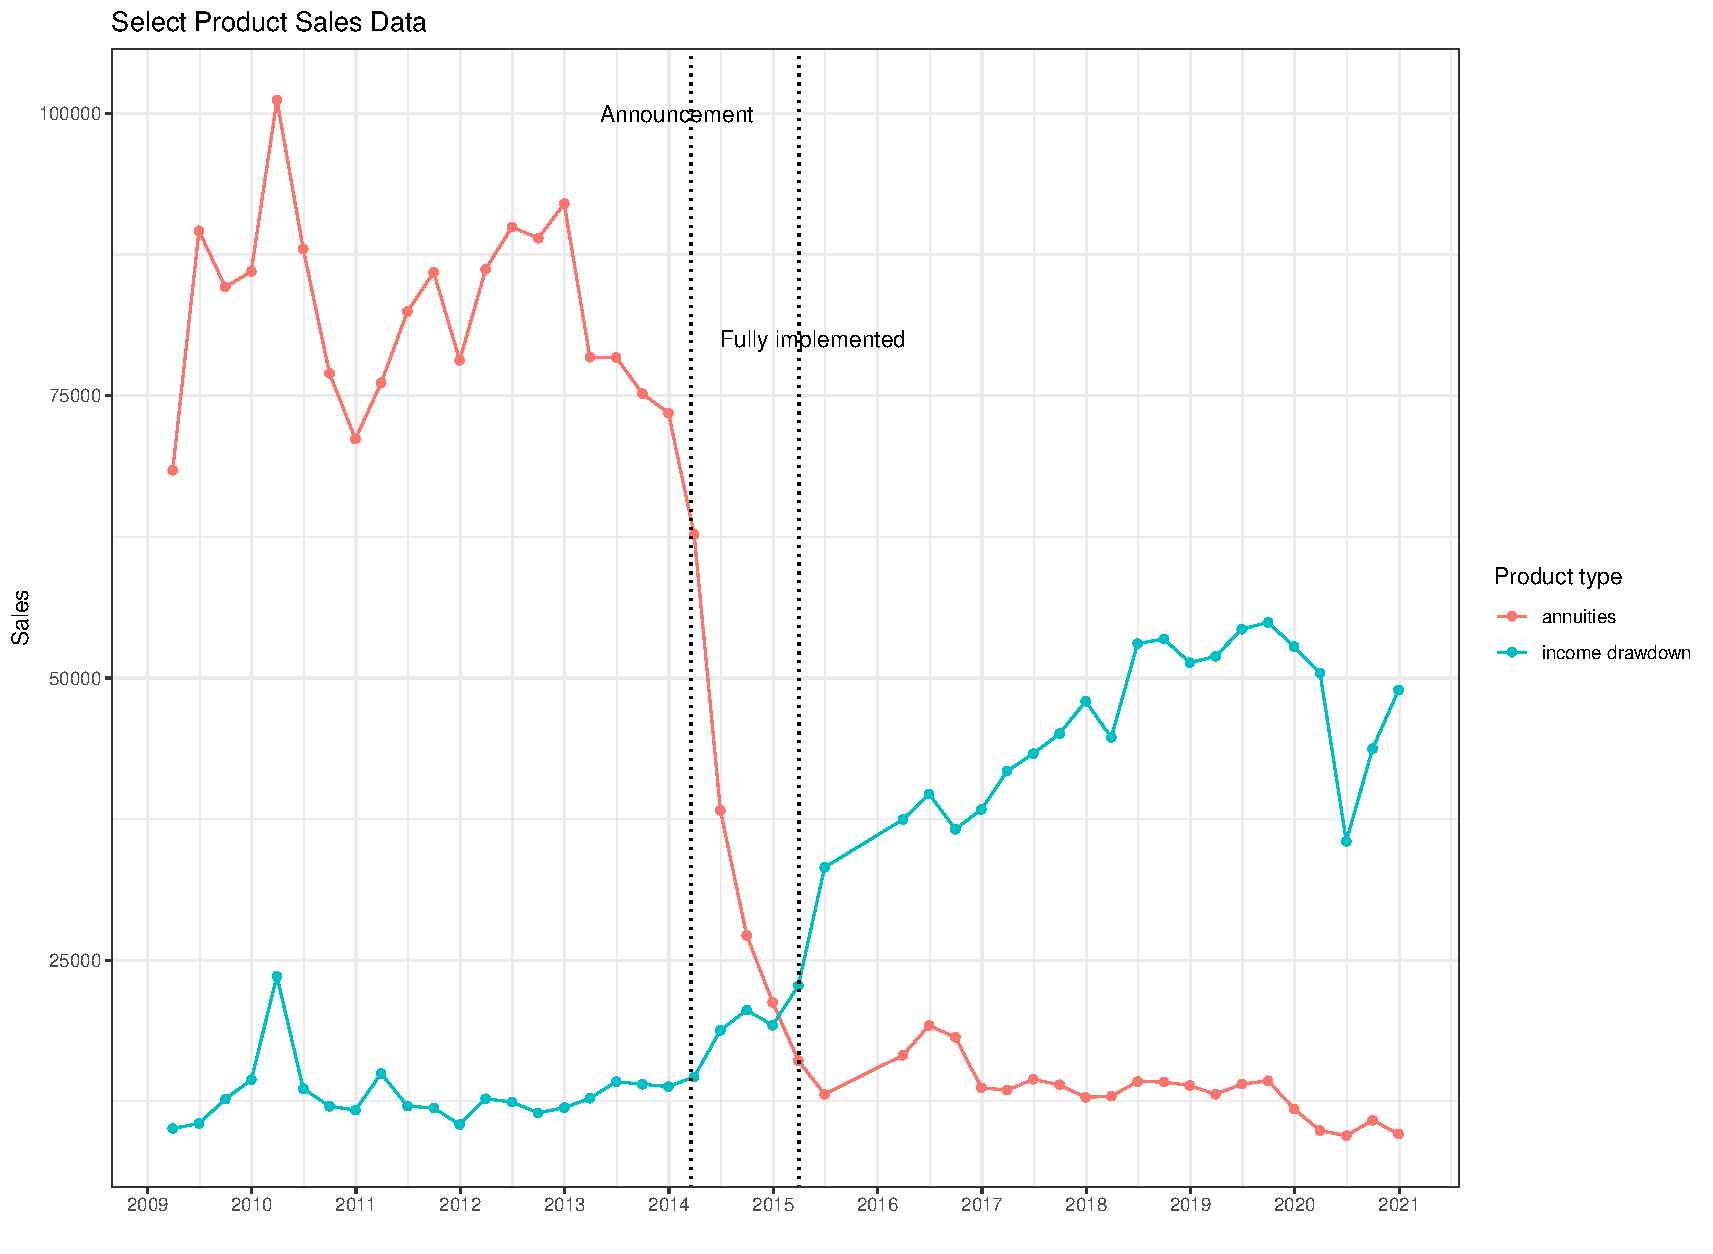
\includegraphics[width=0.7\columnwidth]{figures/annuity_overtime.pdf}
    \label{fig:annovertime}


\end{figure}


\begin{figure}[h]
    \caption[Caption for LOF]{How pension pots are accessed\protect\footnotemark}
    \centering
    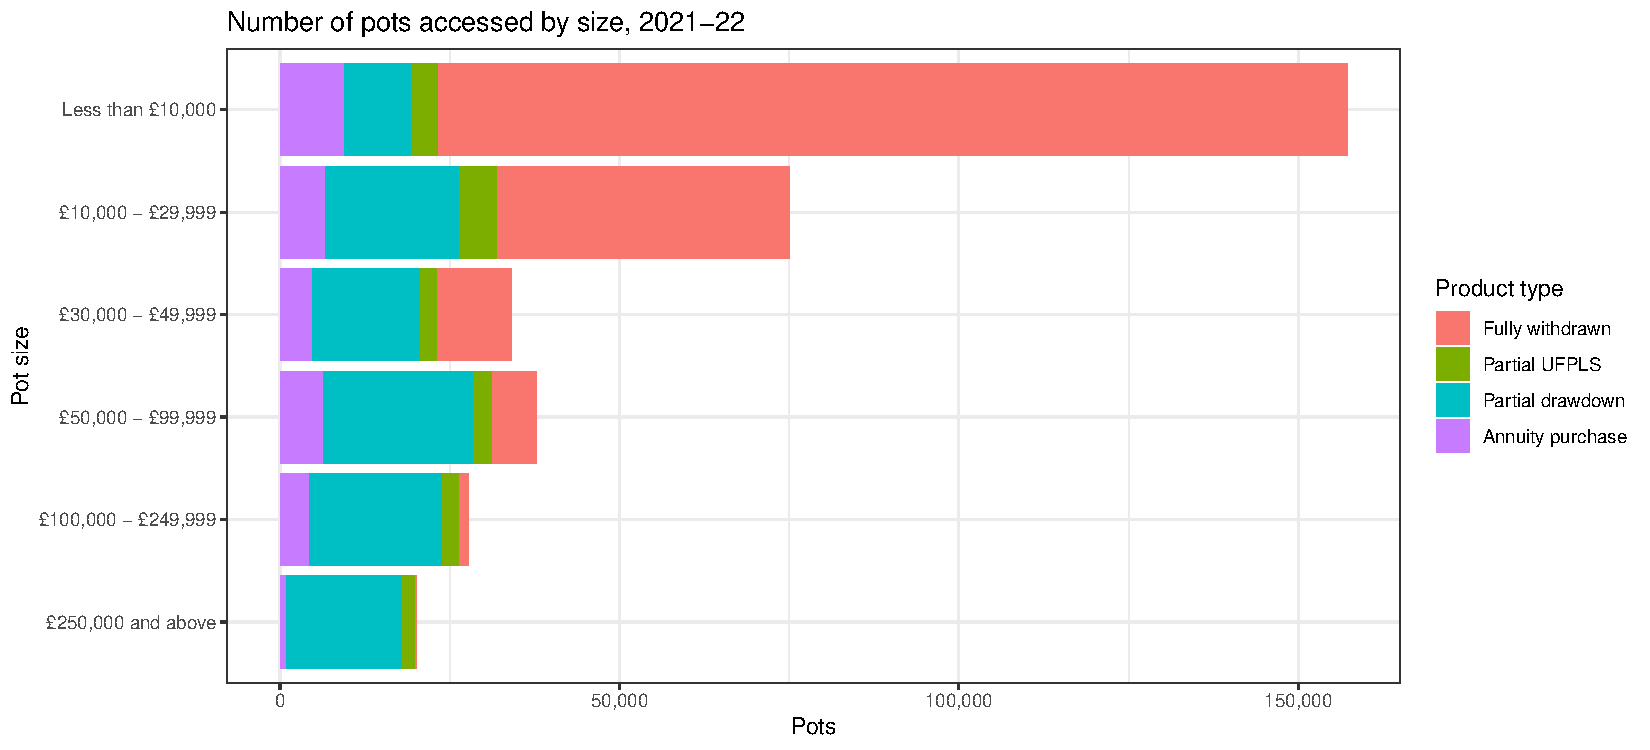
\includegraphics[width=0.7\columnwidth]{figures/annuity_pot_sizes.pdf}
    \label{fig:ann2122}
    \
\end{figure}
Figure \ref{fig:ann2122} shows the distribution of how pension pots were first accessed at retirement in 2021-22.
In 2021, 196,736 pots were fully withdrawn at retirement, accounting for over 50\% of pots. Prior to the policy
reform this was not the case -- most defined contribution pensions were accessed through annuities.
\footnotetext{Partial UFPLS (uncrystallised funds pension lump sum) is similar to Partial drawdown but with a different tax schedule. With partial drawdown
    you take the whole 25\% tax free amount at once whereas with UFPLS you only claim the 25\% on the amount you are taking out. This option is
    better if you may want to buy another retirement product in the future such as an annuity. }


Also of specific interest to the annuity market was the European Union's
`Equal Treatment in Goods and Services Directive' of 2004. This prohibited discrimination
in the provision and cost of goods and services based on sex. Up until 2011, there was a clause that
stated insurers were allowed to charge different premiums if it was based on evidence that sex is
correlated with different amounts of risk. However, in March 2011, the European Court of Justice
ruled that insurers were not allowed to charge different amounts and gave them until December 2012
to implement the ruling. This change meant that annuity products could no longer be priced differently
for men and women in the UK. However, given that this change was implemented two years before the pension
freedoms act, I can still identify the impact of the pensions freedom act on early retirement consumption.

\subsection{Covariate Balance}

Table \ref{tab:sum_stats} shows various summary statistics for each variable of interest from ELSA and the ONS.

As required, retirement year is between 2011 and 2013 for the control group and 2015 and 2017 for the treatment group.
However, as discussed above their interview date is after or the same as the retirement year because we are tracking
consumption in retirement.

The second retirement group, those who retired post reform, is small with just 728 non missing observations for gender as opposed
to 941 individuals in the control group. The control group are more female, retired at a slightly younger age and expected to
retire slightly earlier. This could be because this period was affected by the increase in the state pension age for
women from age 60 in 2010 to age 65 in 2018. Since this change happened gradually and occured over the whole period
I do not expect it to influence the results. The DifferenceAge row tracks the difference between expected and actual
pension age.

The treatment group has higher financial wealth with a median of £66,000 at time of interview as opposed to £55,000
in the control group. Likewise, the second group are more likely to have held a DC pension at some point
and have much more money in them. Both groups are equally likely to have a defined benefit pension with roughly 44\% of
individuals across both samples having a defined benefit pension. In general, DB pensions are more prevalent than
DC pensions in the data, this reflects the same trend that is observed in population of UK retiree. Home ownership
is roughly equal across groups although the second group have slightly higher housing wealth.
\textbf{I have
    not inflation adjusted but I am thinking about it?}

Both groups are similarly long-lived according when using ONS life tables to calculate life expectancy
based on gender, age and the year the interview was carried out in. Subjective life expectancies are also similar
across groups, with individuals expecting to live another 21 years as opposed to the 24 that the ONS would expect
them to live.
\textbf{Maybe add in prob of survival to age 85 or 90 or something}
\textbf{Also add in an indicator for living alone or living with someone else}

Unfortunately, some consumption data is missing for some individuals. The food categories have the least missing data
and the leisure consumption category has the most missing data.

\textbf{Check why total consumption adds up to so much
    more than all the categories added together? Do they include rent and housing in consumption?}


Overall, the groups appear to have slightly different wealth profiles with the treatment group being richer and slightly more likely
to have DC pension wealth. On key demographic characteristics, however, the groups are similar, the difference in retirement
age between the two groups can be mostly explained by the difference in expected retirement age meaning that individuals
have not en masse decided to delay retirement and avoid annuitisation.



\begin{landscape}

    \begin{table}

\caption{Summary statistics \label{tab:sum_stats} }
\centering
\fontsize{10}{12}\selectfont
\begin{tabular}[t]{lrrrrrrrrrr}
\toprule
\multicolumn{1}{c}{ } & \multicolumn{2}{c}{Max} & \multicolumn{2}{c}{Mean} & \multicolumn{2}{c}{Median} & \multicolumn{2}{c}{Min} & \multicolumn{2}{c}{Non Missing} \\
\cmidrule(l{3pt}r{3pt}){2-3} \cmidrule(l{3pt}r{3pt}){4-5} \cmidrule(l{3pt}r{3pt}){6-7} \cmidrule(l{3pt}r{3pt}){8-9} \cmidrule(l{3pt}r{3pt}){10-11}
 & Control & Treat & Control & Treat & Control & Treat & Control & Treat & Control & Treat\\
\midrule
Gender & 1.0 & 1.0 & 0.470 & 0.495 & 0.0 & 0.0 & 0.0 & 0.0 & 753 & 301\\
RetirementYear & 2013.0 & 2017.0 & 2011.875 & 2015.389 & 2012.0 & 2015.0 & 2011.0 & 2015.0 & 753 & 301\\
InterviewYear & 2016.0 & 2017.0 & 2013.328 & 2016.326 & 2014.0 & 2016.0 & 2011.0 & 2015.0 & 753 & 301\\
YearsSinceRetirement & 2.0 & 2.0 & 1.057 & 0.528 & 1.0 & 1.0 & 0.0 & 0.0 & 753 & 301\\
RetiredAge & 82.0 & 79.0 & 63.052 & 63.877 & 63.0 & 64.0 & 55.0 & 55.0 & 753 & 301\\
\addlinespace
AgeAtInterview & 83.0 & 79.0 & 64.109 & 64.405 & 64.0 & 64.0 & 55.0 & 55.0 & 753 & 301\\
ExpectedRetiredAge & 120.0 & 120.0 & 62.317 & 62.773 & 60.0 & 60.0 & 54.0 & 50.0 & 605 & 264\\
DifferenceAge & 48.0 & 44.0 & -0.660 & -0.981 & -1.0 & -1.0 & -8.0 & -22.0 & 605 & 264\\
FinWealth(£000s) & 1.9 & 2.0 & 0.122 & 0.168 & 0.1 & 0.1 & -0.0 & -0.0 & 738 & 297\\
DCPension & 1.0 & 1.0 & 0.198 & 0.259 & 0.0 & 0.0 & 0.0 & 0.0 & 753 & 301\\
\addlinespace
DCValue(£000s) & 8.2 & 17.3 & 0.073 & 0.116 & 0.0 & 0.0 & 0.0 & 0.0 & 684 & 259\\
DBPension & 1.0 & 1.0 & 0.466 & 0.455 & 0.0 & 0.0 & 0.0 & 0.0 & 753 & 301\\
StatePension & 0.0 & 0.0 & 0.005 & 0.005 & 0.0 & 0.0 & 0.0 & 0.0 & 750 & 298\\
OwnsHouse & 1.0 & 1.0 & 0.875 & 0.880 & 1.0 & 1.0 & 0.0 & 0.0 & 753 & 301\\
HouseValue(£000s) & 1.3 & 1.7 & 0.230 & 0.296 & 0.2 & 0.2 & 0.0 & -0.1 & 753 & 301\\
\addlinespace
ObjectiveLifeExp & 33.7 & 34.1 & 23.732 & 23.904 & 23.9 & 23.5 & 7.9 & 10.8 & 753 & 301\\
SubjectiveLifeExp & 36.6 & 37.9 & 20.898 & 20.950 & 21.3 & 21.2 & 4.6 & 5.3 & 527 & 198\\
TotalConsump & 2925.1 & 3495.7 & 729.239 & 780.975 & 647.6 & 699.5 & 130.2 & 136.9 & 753 & 301\\
FoodConsump & 1938.1 & 1938.1 & 415.753 & 425.780 & 363.3 & 373.8 & 51.5 & 36.1 & 748 & 296\\
FoodConsumpIn & 440.0 & 400.0 & 79.964 & 77.706 & 70.0 & 70.0 & 10.0 & 1.0 & 749 & 296\\
\addlinespace
FoodConsumpOut & 750.0 & 1200.0 & 68.302 & 88.208 & 50.0 & 50.0 & 0.0 & 0.0 & 752 & 298\\
ClothingConsump & 1450.0 & 2000.0 & 89.224 & 83.824 & 45.0 & 40.0 & 0.0 & 0.0 & 753 & 301\\
LeisureConsump & 530.0 & 150.0 & 82.072 & 75.000 & 60.0 & 75.0 & 0.0 & 0.0 & 657 & 2\\
UtilityConsump & 483.1 & 580.9 & 107.840 & 113.324 & 96.0 & 100.0 & 0.0 & 0.0 & 753 & 301\\
\bottomrule
\end{tabular}
\end{table}


\end{landscape}


As a further test for balance I regress demographic and financial characteristics of individuals on year of birth and the treatment dummy.
We can then see if the treatment groups differ on key characteristics such as financial wealth or retirement age.
For a regression discontinuity to be valid we need the treatment and control groups to be similar along
all other characteristics apart from the treatment variable.

In particular I run:
\begin{equation*}
    Y_{i} = \alpha + \beta Post_{i} + \gamma YOB_{i} + \kappa (Post_{i} \times YOB_{i}) + \epsilon_{i}
\end{equation*}


\begin{table}

\caption{Covariate Balance \label{tab:cov_balance}}
\centering
\begin{tabular}[t]{lll}
\toprule
 & Pt. est. & SE\\
\midrule
Gender & 2.243 & 10.468\\
RetirementYear & -12.528 & 16.127\\
InterviewYear & -11.243 & 24.959\\
YearsSinceRetirement & 9.716 & 16.056\\
RetiredAge & -12.528 & 16.127\\
\addlinespace
ExpectedRetiredAge & -240.427 & 129.345\\
DifferenceAge & -246.763 & 128.979\\
FinancialWealth (thousands) & -4769.638 & 5410.054\\
DCPension & -13.608 & 8.933\\
DCValue (thousands) & -1978.144 & 20284.768\\
\addlinespace
DBPension & 7.974 & 10.386\\
OwnsHouse & -0.697 & 6.968\\
HouseValue (thousands) & 6630.186 & 4775.236\\
ObjectiveLifeExp & 13.086 & 30.559\\
SubjectiveLifeExp & 0.351 & 182.705\\
\bottomrule
\end{tabular}
\end{table}

Table \ref{tab:cov_balance} shows these results. We can see that being in the treatment group.
\textbf{I am still thinking about this.}


One threat to validity is manipulation of the running variable -- which is the variable that decides
whether an individual is in the treatment group or not -- in our case retirement year.
This is probably quite a threat in this setting as individuals could delay retirement and/or
the purchase of an annuity until after the reform. To check whether
this is happening we see whether the difference between real retirement age and the first expected retirement age
recorded in the data are different for those retiring before 2014 compared to those retiring after 2014. As shown
above in Table \ref{tab:sum_stats} this not the case.

However, it is possible that individuals do not buy an annuity at the time of retirement since the law prior to 2014 only
required that they access the pot by age 75. They may decide to keep their DC pension untouched
and live off other income and assets before accessing it later. Since we do not have data on the
exact purchase date of annuities we cannot track whether
annuity purchases were delayed because of this. However, there is relatively stable annuity demand
before the policy reform. If individuals delayed annuity purchases in expectation of the reform we
would observe declines in purchases before the reform was announced.


\section{Empirical models}

In this section I outline the key empirical models I run with both the simulated consumption data from the
lifecycle models and with the real data from ELSA. I then see which lifecycle model better fits the consumption
response that occurred as a result of the pension reform.

I use a regression discontinuity design for which I compare the consumption of early retirees after the policy reform
to that of people who retired just before the policy reform. The key assumption implicit in regression discontinuities is
that nothing else changes at the time of the jump apart from the policy of interest, and that the policy occurs
without individuals predicting it and altering their behaviour. As I have argued above, the demographic information in the
data suggest that individuals did not delay retirement and that there was no delay in annuitisation as shown by the quick
and sudden decline in annuity purchases. Moreover, anecdotal evidence from media and business sources at the time of the
announcement show that there was surprise the government had gone this far, with money marketing describing the change as a
"bombshell" \cite{money_marketing_announcement}.

Retirement year is the running variable and individuals are treated if retirement year is greater than 2014 and less than
or equal to 2017. I use consumption data of individuals up to 2 years into retirement so that the sample size is larger.
So if someone retired in 2015 and had consumption data in 2015 and 2017, I include both values. An individual is considered
not treated if they retire before 2013 and after 2011.  To account for the fact
that the reform only impacted individuals who had accumulated defined contribution pension pots I interact the treatment dummy with
an indicator variable signalling whether the individual had ever held a DC pension pot.

Because of the differences in financial characteristics between the groups, I add controls for financial wealth, housing wealth
and whether an individual owns their own home.

\begin{equation*}
    Cons_{it} =  \gamma X_{it} + \beta PostReform_{it} + \epsilon
\end{equation*}

And $X_{it}$ is a set of controls.

\begin{landscape}
    \begin{table}

\caption{DC Only \label{tab:DcOnlyRes}}
\centering
\begin{tabular}[t]{lddddd}
\toprule
  & {TotalConsump} & {FoodConsump} & {FoodConsumpIn} & {FoodConsumpOut} & {ClothingConsump}\\
\midrule
(Intercept) & 1021.473 & 336.236 & 51.012 & 111.948 & -40.948\\
 & (311.124) & (88.870) & (37.892) & (76.345) & (288.889)\\
PostReform & -263.566 & 28.985 & 18.670 & -49.062 & -51.413\\
 & (16.736) & (8.018) & (5.111) & (13.483) & (34.475)\\
rv & 81.454 & -5.037 & -4.324 & 13.410 & -8.369\\
 & (2.204) & (1.906) & (0.365) & (3.358) & (3.877)\\
RetiredAge & 0.668 & 0.215 & 0.126 & -0.314 & 0.635\\
 & (5.180) & (1.061) & (0.641) & (1.734) & (4.967)\\
FinWealth(£000s) & 0.245 & 0.143 & 0.006 & 0.108 & -0.019\\
 & (0.122) & (0.015) & (0.002) & (0.014) & (0.030)\\
Gender & -39.881 & -34.203 & -8.601 & 2.464 & 10.879\\
 & (34.523) & (14.191) & (1.892) & (20.927) & (36.216)\\
DCValue(£000s) & -0.016 & 0.006 & 0.002 & -0.004 & -0.006\\
 & (0.006) & (0.007) & (0.001) & (0.003) & (0.002)\\
YearsSinceRetirement & 27.491 & -7.975 & -1.441 & -2.648 & 12.890\\
 & (20.390) & (8.144) & (2.536) & (2.633) & (5.426)\\
OwnsHouse & -115.386 & 118.737 & 25.877 & 7.199 & 81.823\\
 & (18.262) & (38.551) & (0.648) & (40.684) & (6.002)\\
StatePension & -12.412 & -4.698 & -0.915 & -0.497 & -3.962\\
 & (2.809) & (2.929) & (0.876) & (0.709) & (7.634)\\
PostReform:rv & 10.776 & -11.726 & -4.714 & 8.585 & 80.550\\
 & (16.406) & (13.998) & (2.851) & (1.129) & (11.147)\\
\midrule
Num.Obs. & 208 & 205 & 205 & 208 & 208\\
R2 & 0.071 & 0.061 & 0.057 & 0.106 & 0.053\\
R2 Adj. & 0.023 & 0.013 & 0.008 & 0.060 & 0.005\\
\bottomrule
\multicolumn{6}{l}{\rule{0pt}{1em}I use robust standard errors clustered at the treatment level
    since standard errors are
    likely correlated within these groups.}\\
\end{tabular}
\end{table}

\end{landscape}


Table \ref{tab:DcOnlyRes} shows the results of this specification on the various consumption indicators.
Column 1 has total monthly consumption on the left hand side of the regression equation.
We can see that being in the treatment group is associated with £73 more a week in spending
overall across all categories of expenditure. This is not statistically significant using
robust standard errors \textbf{find a reference for the SE that I use}. Being further into retirement
at the time of interview is also associated with lower consumption whilst those who retired later have lower consumption
because years since the start of retirement is associated with higher total consumption.

Columns 2 through 4 use food consumption as the outcome variable. Interestingly, food consumption
inside the house does not increase as a result of the policy reform but food consumed away from the house does
increase. If individuals see their pension pot, that they previously could not access, as a
shock to their wealth, like winning the lottery, then we would expect the consumption basket to
include more goods that are perceived as luxuries. Inline with this, consumption on clothing, shown in
column 4, increases as a result of the policy change.

One concern is that the group who retired after 2014 are just generally different to those
who retired before and perhaps consume more outside the home anyway. The financial characteristic
data presented in \ref{tab:sum_stats} would support this hypothesis. To test for these cohort
effects I run a difference in difference regression to complement the regression discontinuity just shown.
I add individuals who have a defined benefit pension pot into the model and interact the policy change
with dummies for having different types of pension. Specifically I run:

\begin{equation*}
    Cons_{it} =  \gamma X_{it} + \beta_{1} PostReform_{it} + \beta_{2} PostReform*DC_{it} + \beta_{3} PostReform*DB_{it}  + \epsilon
\end{equation*}


This makes the coefficient of interest $\beta_{2}$, which shows us the difference
in the change in consumption between the DC only group and the base group that has neither a DB or DC pension.
Since rules for DB pensions did not change under the pensions freedom act, those with a DB pension or no pension
can be seen as a natural counterfactual group to judge the consumption of the DC group against.

\begin{landscape}
    \begin{table}

\caption{All individuals with interaction \label{tab:ElsaAllData}}
\centering
\begin{tabular}[t]{lddddd}
\toprule
  & {TotalConsump} & {FoodConsump} & {FoodConsumpIn} & {FoodConsumpOut} & {ClothingConsump}\\
\midrule
(Intercept) & 588.449 & 376.400 & 81.643 & 23.591 & 129.552\\
 & (140.286) & (31.367) & (12.656) & (85.192) & (35.146)\\
PostReform & 94.121 & 14.164 & -1.591 & 21.122 & -1.439\\
 & (4.541) & (0.419) & (0.335) & (1.215) & (0.657)\\
DCPension & 48.471 & 29.337 & 3.056 & 15.300 & -3.224\\
 & (4.408) & (2.544) & (0.503) & (0.260) & (1.616)\\
DBPension & 90.885 & 16.998 & -0.356 & 18.744 & 22.568\\
 & (2.243) & (5.906) & (0.190) & (5.217) & (1.797)\\
RetiredAge & 2.320 & -0.781 & -0.218 & 0.140 & -1.609\\
 & (2.643) & (0.136) & (0.272) & (1.301) & (0.867)\\
FinWealth(£000s) & 0.166 & 0.072 & -0.002 & 0.080 & 0.017\\
 & (0.009) & (0.028) & (0.006) & (0.005) & (0.013)\\
Gender & -19.453 & -19.704 & -5.024 & 2.024 & -0.014\\
 & (9.136) & (26.358) & (4.913) & (4.729) & (2.243)\\
DCValue(£000s) & -0.012 & 0.004 & 0.002 & -0.003 & -0.004\\
 & (0.000) & (0.009) & (0.002) & (0.002) & (0.002)\\
YearsSinceRetirement & 37.784 & -10.041 & -2.018 & -1.564 & 6.843\\
 & (10.397) & (0.877) & (0.992) & (3.449) & (1.411)\\
OwnsHouse & -90.415 & 110.119 & 20.541 & 20.923 & 42.791\\
 & (27.860) & (2.329) & (2.187) & (7.207) & (5.948)\\
StatePension & -5.971 & -2.925 & -0.445 & -0.957 & 0.669\\
 & (3.949) & (2.058) & (0.416) & (0.269) & (2.020)\\
PostReform:DCPension & 12.823 & -4.930 & -0.463 & -2.085 & 37.406\\
 & (3.134) & (0.311) & (0.172) & (0.262) & (0.411)\\
PostReform:DBPension & -139.946 & -24.437 & -1.744 & -16.814 & -15.134\\
 & (2.228) & (0.024) & (0.290) & (1.385) & (0.565)\\
\midrule
Num.Obs. & 926 & 917 & 918 & 923 & 926\\
R2 & 0.039 & 0.049 & 0.031 & 0.105 & 0.029\\
R2 Adj. & 0.027 & 0.036 & 0.018 & 0.093 & 0.016\\
\bottomrule
\multicolumn{6}{l}{\rule{0pt}{1em}I use robust standard errors clustered at the treatment level
    since standard errors are
    likely correlated within these groups.}\\
\end{tabular}
\end{table}

\end{landscape}

Table \ref{tab:ElsaAllData} shows these results. The post reform variable
now tells us that total consumption decreased but food consumption increased a little and clothing consumption
decreased. The interactions at the bottom of the table show us what happened to individuals with a given pension
type relative to the reference cohort which has no pension. Those with only a DC pension had an increase in total consumption
which was lower than that for those with a DB pension but higher than those with no pension. Only for consumption on
clothes did DC consumption increase more than the other groups. As above, the only variables that are significant
at the 5\% level are financial wealth and whether the individual owns their house.

We can also test whether treatment intensity is correlated with larger increases in spending. Those who have
more money in a DC pension, and those with more financial wealth overall, would be impacted
by the policy to a greater extent than those with smaller pensions. So, I interact the policy with the treatment
variable. As in Table \ref{tab:DcOnlyRes}, this regression only uses those individuals who have a DC pension.

To be precise I run:
\begin{equation*}
    Cons_{it} =  \gamma X_{it} + \beta PostReform_{it}*DCValue_{it} + \epsilon
\end{equation*}

\begin{landscape}
    \begin{table}

\caption{DC Pension Size interaction \label{tab:DcOnlyInteract}}
\centering
\begin{tabular}[t]{lccccc}
\toprule
  & TotalConsump & FoodConsump & FoodConsumpIn & FoodConsumpOut & ClothingConsump\\
\midrule
(Intercept) & \num{1347.198} & \num{571.090} & \num{77.009} & \num{220.315} & \num{40.944}\\
 & (\num{745.238}) & (\num{346.747}) & (\num{68.914}) & (\num{122.712}) & (\num{217.875})\\
PostReform & \num{74.604} & \num{9.797} & \num{0.123} & \num{11.064} & \num{27.427}\\
 & (\num{69.978}) & (\num{27.205}) & (\num{5.366}) & (\num{9.226}) & (\num{24.871})\\
RetiredAge & \num{-4.652} & \num{-3.172} & \num{-0.073} & \num{-2.585} & \num{-0.295}\\
 & (\num{10.447}) & (\num{5.435}) & (\num{1.089}) & (\num{1.893}) & (\num{3.609})\\
FinancialWealth (thousands) & \num{0.229} & \num{0.172} & \num{0.013} & \num{0.111} & \num{-0.012}\\
 & (\num{0.114}) & (\num{0.050}) & (\num{0.010}) & (\num{0.025}) & (\num{0.053})\\
Gender & \num{-19.457} & \num{-35.355} & \num{-6.937} & \num{-6.007} & \num{13.359}\\
 & (\num{63.228}) & (\num{28.103}) & (\num{5.502}) & (\num{10.149}) & (\num{24.880})\\
DCValue (thousands) & \num{-0.009} & \num{0.022} & \num{0.006} & \num{-0.004} & \num{-0.002}\\
 & (\num{0.027}) & (\num{0.035}) & (\num{0.008}) & (\num{0.004}) & (\num{0.009})\\
YearsSinceRetirement & \num{-1.902} & \num{-7.906} & \num{-0.268} & \num{-7.741} & \num{6.092}\\
 & (\num{44.666}) & (\num{16.767}) & (\num{3.225}) & (\num{6.186}) & (\num{14.714})\\
OwnsHouse & \num{-261.541} & \num{101.085} & \num{20.990} & \num{10.656} & \num{73.604}\\
 & (\num{196.144}) & (\num{37.911}) & (\num{7.293}) & (\num{14.787}) & (\num{16.328})\\
StatePension & \num{-14.040} & \num{-4.125} & \num{-1.256} & \num{1.258} & \num{-3.040}\\
 & (\num{9.566}) & (\num{4.105}) & (\num{0.841}) & (\num{1.265}) & (\num{4.052})\\
PostReform:DCValue (thousands) & \num{-0.003} & \num{-0.022} & \num{-0.005} & \num{0.000} & \num{-0.002}\\
 & (\num{0.045}) & (\num{0.035}) & (\num{0.008}) & (\num{0.004}) & (\num{0.017})\\
\midrule
Num.Obs. & \num{209} & \num{326} & \num{326} & \num{330} & \num{221}\\
R2 & \num{0.068} & \num{0.066} & \num{0.051} & \num{0.102} & \num{0.035}\\
R2 Adj. & \num{0.026} & \num{0.039} & \num{0.024} & \num{0.076} & \num{-0.006}\\
AIC & \num{3156.1} & \num{4500.7} & \num{3452.4} & \num{3836.7} & \num{2897.0}\\
BIC & \num{3192.9} & \num{4542.4} & \num{3494.1} & \num{3878.5} & \num{2934.4}\\
Log.Lik. & \num{-1567.065} & \num{-2239.361} & \num{-1715.225} & \num{-1907.357} & \num{-1437.504}\\
RMSE & \num{436.58} & \num{232.82} & \num{46.64} & \num{78.33} & \num{161.68}\\
Std.Errors & HC3 & HC3 & HC3 & HC3 & HC3\\
\bottomrule
\end{tabular}
\end{table}

\end{landscape}

Table \ref{tab:DcOnlyInteract} shows the results. Surprisingly, a larger DC pension
pot is not associated with a greater increase in consumption. And although the reform is again associated with an
increase in consumption, especially for food out of the house and clothing, this affect is decreasing with the
size of the pension pot.


The defined contribution pension pot size variable comes from work done by the IFS. This was discontinued
after wave 5 so it is no longer possible to identify pension wealth in this way. For the above table pension
wealth from the last available year for an individual was given a real return of 3\% and compounded until year of interview.
Given that this is an imperfect measure, I also run the regression with financial wealth interacted with the treatment variable.

\begin{landscape}
    \begin{table}

\caption{DC Financial Wealth interaction \label{tab:DcOnlyFinWealthInteract}}
\centering
\begin{tabular}[t]{lddddd}
\toprule
  & {TotalConsump} & {FoodConsump} & {FoodConsumpIn} & {FoodConsumpOut} & {ClothingConsump}\\
\midrule
(Intercept) & 792.453 & 157.868 & 56.231 & -89.273 & 110.932\\
 & (380.887) & (479.454) & (55.927) & (238.508) & (241.514)\\
PostReform & 77.996 & 9.980 & -2.599 & 20.981 & 30.043\\
 & (3.083) & (6.929) & (0.644) & (9.406) & (8.346)\\
RetiredAge & 2.134 & 4.024 & 0.201 & 3.187 & -1.370\\
 & (3.940) & (8.389) & (0.919) & (4.432) & (4.258)\\
FinWealth(£000s) & 0.322 & 0.164 & 0.009 & 0.117 & 0.059\\
 & (0.068) & (0.001) & (0.003) & (0.011) & (0.026)\\
Gender & -31.169 & -47.768 & -8.490 & -11.772 & 8.354\\
 & (33.636) & (21.976) & (2.569) & (31.747) & (32.934)\\
YearsSinceRetirement & 0.541 & -23.842 & -2.771 & -12.460 & -11.846\\
 & (8.561) & (1.625) & (4.359) & (16.759) & (4.174)\\
OwnsHouse & -139.190 & 102.073 & 25.433 & -8.030 & 74.816\\
 & (121.783) & (6.659) & (2.061) & (2.063) & (1.233)\\
StatePension & -15.442 & -7.971 & -0.775 & -4.373 & -0.596\\
 & (9.403) & (7.492) & (1.175) & (2.615) & (7.285)\\
PostReform:FinWealth(£000s) & 0.098 & -0.025 & -0.003 & -0.002 & -0.116\\
 & (0.064) & (0.015) & (0.001) & (0.015) & (0.030)\\
\midrule
Num.Obs. & 222 & 219 & 219 & 222 & 222\\
R2 & 0.077 & 0.072 & 0.048 & 0.088 & 0.030\\
R2 Adj. & 0.042 & 0.037 & 0.012 & 0.054 & -0.007\\
\bottomrule
\multicolumn{6}{l}{\rule{0pt}{1em}I use robust standard errors clustered at the treatment level
    since standard errors are
    likely correlated within these groups.}\\
\end{tabular}
\end{table}

\end{landscape}

Table \ref{tab:DcOnlyFinWealthInteract} contains these results and shows a similar pattern to Table \ref{tab:DcOnlyInteract}.
The reform is associated with an increase in consumption, but more financial wealth decreases the effect rather
than making it stronger. This could be because those with higher levels of financial wealth have more assets in
other savings apart from retirement savings \cite{cribb_karjalainen_ifs_2023} and therefore the DC pot is a smaller proportion of overall assets,
and thus the policy change did not affect them as much.

In conclusion, the results in the tables above show that in the basic regression discontinuity setup there is
an impact of the policy reform on consumption, and this effect is stronger for consumption goods we
would associate with a large increase in income. However, this is imprecisely estimated, and when we use a
difference in difference identification method this effect disappears. Moreover, when we interact with a proxy for treatment strength
(financial wealth or pension size) the effect is smaller the stronger the treatment.

Theoretically, a null change in consumption is evidence for a bequest motive explaining a lack of annuitisation
rather than pessimistic life expectancies being the cause. In the next section I simulate a lifecycle model
for individuals in the ELSA dataset and
\textbf{some thing that gives a taster of the results to come in the next section}



\section{Life cycle theory}

In the second part of the paper I first solve a modified retirement lifecycle model and then use data from the solved lifecycle
model in similar regressions to the ones above.

The problem that retirees face is as follows. Every period retirees solve:

\begin{equation*}
    V_{t}(a_{t}, y) = \underset{a_{t+1}, c_{t}}{\max} \{ u(c_{t}) + p_{t}B(a_{t+1}) + \beta(1-p_{t})V_{t+1}(a_{t+1}, y) \}
\end{equation*}

subject to their budget constraint

\begin{equation*}
    c_{t} =a_{
    t}(1 +r) -  a_{t+1} + y
\end{equation*}

where $a_{t}$ are asset holdings in time t, $y$ is constant income for all periods, $V_{t}$ is value in period $t$, $p_{t}$ is probability of
death in period $t$ and $B()$ is a bequest function. Income can come either
from state pensions, defined benefit pension plans or purchased annuities.

\begin{equation*}
    u(c_{t}) = \frac{c_{t}^{1 - \sigma}}{1 - \sigma}
\end{equation*}

In some specifications retirees can leave bequests, I use the bequest function from
\cite{lockwood_red_2012}.

\begin{equation*}
    B(a_{t+1}) = \bigl( \frac{m}{1 - m} \bigr)^{\sigma}  \frac{(\frac{m}{1 - m}c_{0} + a_{t+1})^{(1 - \sigma)}}{1 - \sigma}
\end{equation*}

Where $a_{t+1}$ is the amount left at death, $m$ is a measure of bequest motive strength and $c_{0}$ is
a minimum amount of consumption that individuals want. I pick values of $m = 0.95$ and $c_{0} = 20,000$ since
these generate low rates of annuitisation, for comparison, Lockwood picks $m = 0.96$ and $c_{0} = 18,000$
\textbf{Check all of this}

First, I discretise the state space. I create a grid from 500 to 50,000 incrementing by 500 for income and 1000 to
500,000 incrementing by 1000 for financial assets. I solve the retirees problem using backward induction. At age 110 there is certainty of death so any leftover assets
are carried over into the next period and bequested. This means that the value at the end of the final period is
either 0 (if we do not allow a bequest motive) or the value of bequests. I then take this value function and solve
an individual's final period problem, choosing assets next period (i.e. those to bequest) and how much to consume.

Using the optimal policy function in the last period, which is assets next period that maximise the utility
function and the value function this period given all the potential income and asset states, I calculate the value of the last period.
This is then used in the problem the year before that.
I repeat this process back to the age of retirement to obtain optimal consumption amounts for each year of retirement
and associated value functions.

To simulate the ELSA data I solve this retirement problem for each new retiree in the data set dependent on their
objective probability of death each period. I estimate with subjective life expectancies and objective life expectancies.
I also estimate the model both with and without a bequest motive which was picked to roughly fit the real annuity
rates seen in the data.

In retiree's first year of retirement I allow them to choose to annuitise some of their wealth. In practical terms
this is moving down the asset grid but up the income grid and seeing if the value of being in that position is better
than where the individual is currently. To assess this trade-off I calculate the annual annuity payment that follows
from a given annuity cost. I calculate this using objective life tables from the ONS using the following equation:

\begin{equation*}
    Ann = \delta * C * \biggl[\sum_{t = Retage}^{110}\frac{1 - p_{t|Retage}}{(1 + r)^{t - Retage}}\biggr]^{-1}
\end{equation*}

Where $C$ is the one-off payment, $\delta$ is a factor that controls the `money's worth' of annuity and $p_{t|Retage}$
is the probability of death at age $t$ conditional on being age $Retage$. So individuals can move C on the asset grid
for gaining Ann on the income grid for the rest of their lives.

I also simulate the expected change in consumption given different rates of annuitisation versus no annuitisation.
The benefit of simulating an individual's decision is that we can directly compare what they would have
consumed with what they actually consumed, and we can replicate the empirical analysis using the
solution to the lifecycle model.

I first round an individuals financial wealth to the nearest point on the discrete asset grid, and
do likewise for an individuals state pension income. I then take the treatment group and evaluate
their consumption in the year of interview with an annuity given that they annuitised some portion
of their wealth in their retirement year. I also evaluate consumption without annuitisation. I then
use the same specification as above, but now the treatment group is the values of consumption without
annuitisation.

Because I discretised the state space, annuity prices are rounded down to the nearest income grid point.
This means that for some individuals with low assets half of their financial wealth does not buy them
at least one grid point of annuity income. I do not let these individuals annuitise, setting consumption
with and without an annuity to the same amount. I also present the average implied loading factor
$\delta$, although I set this to $0.9$ when calculating annuity prices, because of rounding down
this is lower.


\begin{landscape}

    \begin{table}

\caption{Simulated standard lifecycle models \label{tab:StandardLifeCycle}}
\centering
\begin{tabular}[t]{ldddd}
\toprule
  & {DCOnly} & {AllDataDCInteraction} & {DCOnlyPensionInt} & {DCOnyFinancialInt}\\
\midrule
(Intercept) & -681.172 & -648.121 & -681.816 & -588.159\\
PostReform & 2.841 & -4.678 & 0.558 & 30.651\\
RetiredAge & 10.688 & 10.332 & 10.714 & 9.088\\
FinWealth(£000s) & 4.433 & 4.316 & 4.435 & 4.512\\
Gender & 13.066 & 23.299 & 12.707 & 14.345\\
DCValue(£000s) & 0.000 & 0.001 & -0.006 & {}\\
YearsSinceRetirement & -6.223 & -0.621 & -6.492 & -7.268\\
OwnsHouse & 14.666 & 21.488 & 15.294 & 13.215\\
StatePension & 89.059 & 89.236 & 89.086 & 89.271\\
DCPension & {} & -15.382 & {} & {}\\
DBPension & {} & 1.522 & {} & {}\\
PostReform:DCPension & {} & 17.764 & {} & {}\\
PostReform:DBPension & {} & -11.353 & {} & {}\\
PostReform:DCValue(£000s) & {} & {} & 0.007 & {}\\
PostReform:FinWealth(£000s) & {} & {} & {} & -0.219\\
\midrule
Num.Obs. & 139 & 584 & 139 & 147\\
R2 & 0.995 & 0.993 & 0.995 & 0.995\\
R2 Adj. & 0.994 & 0.993 & 0.994 & 0.995\\
\bottomrule
\end{tabular}
\end{table}

\end{landscape}

Table \ref{tab:StandardLifeCycle} shows the results from the bequest models.



\begin{landscape}
    \begin{table}

\caption{Simulated bequest lifecycle models \label{tab:BeqLifeCycle}}
\centering
\begin{tabular}[t]{lcccc}
\toprule
  & DCOnly & AllDataDCInteraction & DCOnlyPensionInt & DCOnyFinancialInt\\
\midrule
(Intercept) & \num{-447.672} & \num{-543.511} & \num{-448.371} & \num{-439.946}\\
PostReform & \num{16.687} & \num{-10.850} & \num{14.207} & \num{24.811}\\
RetiredAge & \num{7.577} & \num{9.155} & \num{7.605} & \num{7.446}\\
FinancialWealth (thousands) & \num{4.076} & \num{4.071} & \num{4.078} & \num{4.103}\\
Gender & \num{13.731} & \num{19.651} & \num{13.342} & \num{13.384}\\
DCValue (thousands) & \num{0.001} & \num{0.001} & \num{-0.005} & \\
YearsSinceRetirement & \num{-1.225} & \num{-0.888} & \num{-1.517} & \num{-2.273}\\
OwnsHouse & \num{5.064} & \num{17.853} & \num{5.746} & \num{3.839}\\
StatePension & \num{84.422} & \num{84.994} & \num{84.451} & \num{84.404}\\
DCPension &  & \num{-20.629} &  & \\
DBPension &  & \num{0.556} &  & \\
PostReform:DCPension &  & \num{25.529} &  & \\
PostReform:DBPension &  & \num{2.655} &  & \\
PostReform:DCValue (thousands) &  &  & \num{0.008} & \\
PostReform:FinancialWealth (thousands) &  &  &  & \num{-0.061}\\
\midrule
Num.Obs. & \num{139} & \num{584} & \num{139} & \num{147}\\
R2 & \num{0.996} & \num{0.995} & \num{0.996} & \num{0.996}\\
R2 Adj. & \num{0.995} & \num{0.995} & \num{0.995} & \num{0.995}\\
AIC & \num{1420.0} & \num{5938.7} & \num{1419.6} & \num{1496.3}\\
BIC & \num{1449.4} & \num{5999.9} & \num{1451.9} & \num{1526.2}\\
Log.Lik. & \num{-700.021} & \num{-2955.338} & \num{-698.814} & \num{-738.142}\\
RMSE & \num{37.23} & \num{38.15} & \num{36.91} & \num{36.69}\\
Std.Errors & HC3 & HC3 & HC3 & HC3\\
\bottomrule
\end{tabular}
\end{table}

\end{landscape}

Table \ref{tab:BeqLifeCycle} shows the results from the bequest models.




Each column in the table shows a different model. Column 1 shows the model with no bequest motive where
individuals use objective life probabilities from ONS, column 2 uses


\textbf{Also get some plots of consumption in early retirement
    with and without annuities for the different model types}





% \subsection{Rough plan}
% \begin{itemize}
%   \item Intro
%         \begin{enumerate}
%           \item I think Eric French wrote something about population that I could use in then intro to say why it is important.
%           \item "Latest data from HM Revenue Customs (published in April) showed more than £45bn has been taken from pots since 2015."
%                 https://www.ftadviser.com/pensions/2022/02/08/pension-freedoms-were-they-really-a-good-idea/


%           \item Add bit about DC/DB pensions in the intro. Also talk about heterogeneity across countries.
%                 Some countries want to move towards more annuitisation. This annual review is a good source of info
%                 \cite{banks_crawford_ar_2022}
%           \item https://www.moneysavingexpert.com/savings/pension-freedom/
%         \end{enumerate}
%   \item Lit review
%   \item Models
%   \item Empirical
%         \begin{enumerate}
%           \item Diff in diff
%           \item RDD
%           \item Matching?
%           \item can I use anything I learnt in panel?
%                 In some sense the decision to annuitise is a discrete choice problem so I could use something from there.
%         \end{enumerate}
%   \item Conclusion
% \end{itemize}



\bibliographystyle{apa}
\bibliography{references}
\end{document}